% Name: Cycle and path
% Description: The cycle C6, six vertices joined in a ring, beside the path P6, the same six vertices in a line with one edge fewer.
% Tags: cycle graph, path graph, graph theory

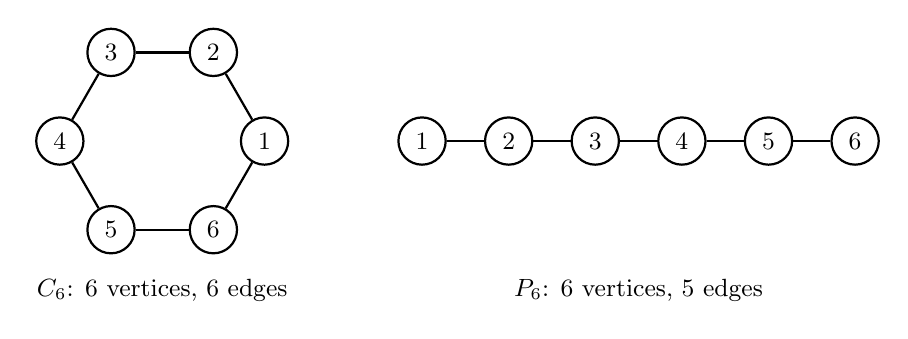
\begin{tikzpicture}[vertex/.style={circle, draw, thick, fill=white, minimum size=6mm, inner sep=0pt, font=\small}]
  % The cycle: vertex i at angle 60(i-1) degrees on a circle of radius 1.3.
  \foreach \i in {1,...,6}
    \node[vertex] (c\i) at ({60*(\i-1)}:1.3) {$\i$};
  \foreach \i [evaluate=\i as \j using {int(mod(\i,6)+1)}] in {1,...,6}
    \draw[thick] (c\i) -- (c\j);
  \node[font=\small] at (0,-1.9) {$C_6$: 6 vertices, 6 edges};

  % The path, to the right.
  \foreach \i in {1,...,6}
    \node[vertex] (p\i) at ({2.2+1.1*\i},0) {$\i$};
  \foreach \i [evaluate=\i as \j using {int(\i+1)}] in {1,...,5}
    \draw[thick] (p\i) -- (p\j);
  \node[font=\small] at (6.05,-1.9) {$P_6$: 6 vertices, 5 edges};
\end{tikzpicture}
